\begin{center}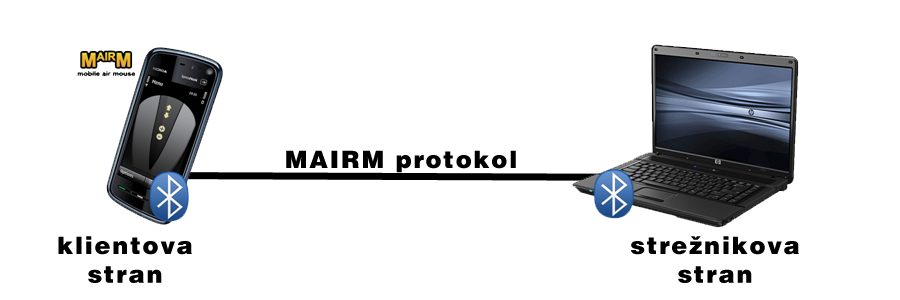
\includegraphics[width=140mm]{images/arch.png}\end{center}
Re�itev je zasnovana s pomo�jo principa stre�nik-odjemalec. Stre�nik in odjemalec med sabo komunicirata preko MAIM protokola, ki je osnovan na JSON formatu ter je predstavljen v nadaljevanju poro�ila.
\newline\newline
Na stre�nikovi (ra�unalnikovi) strani te�e MAIRM stre�ni�ka aplikacija. Njene naloge so:
\begin{itemize}
\item ustvari bluetooth service (z imenom MAIRM) preko katerega se MAIRM odjemalec pove�e do same aplikacije,
\item poskrbi za pravilno prepoznavo odjemal�evih akcij:
	\begin{itemize}
		\item premikanje mi�ke po zaslonu,
		\item pomikanje po straneh (scrolling),
		\item uporaba mobilne tipkovnice,
		\item prepoznavanje 3D kretenj
	\end{itemize}
\item skrbi za pravilen odziv glede na odjemal�evo akcijo:
	\begin{itemize}
		\item �e zazna zahtevo po premiku mi�ke, premakne mi�ko
		\item �e zazna zahtevo po pomikanje preko strani, simulira potreben dogodek
		\item �e zazna zahtevo po pritisku tipke, simulira pritisk
		\item �e zazna 3D kretnjo naredi akcijo (akcija je dolo�ena v XML datoteki), ki je dolo�ena za njo:
			\begin{itemize}
				\item po�ene nek program
				\item pritisne neko kombinacijo tipk
			\end{itemize}
	\end{itemize}
\end{itemize}
Na mobitelovi strani oziroma odjemal�evi strani te�e MAIRM odjemal�eva aplikacija. Njene naloge so:
\begin{itemize}
\item zajemanje podatkov iz merilnika pospe�ka vgrajenega v sam mobitel,
\item zajemanje pritiskov tipk,
\item posredovanje zajetih podatkov po MAIRM protokolu vse do MAIRM stre�ni�ke aplikacije,
\item skrbi za preklapljanje med naslednjimi na�ini delovanja:
	\begin{itemize}
		\item Mouse mode,
		\item Scrolling mode,
		\item Gesture mode
	\end{itemize}
\item izris uporabni�kega vmesnika za touch screen telefone.
\end{itemize}
Obe komponenti sistema skupaj tvorita delujo�o osnova s katero se (lahko) dose�e zastavljene za�etne cilje.
\subsection{MAIRM protokol}
Sam protol je v JSON formatu in te�e preko Bluetooth Serial Port ter je zelo enostaven. V trenutni verziji je podprta samo enosmerna komunikacija.
\subsubsection{Uporabljeni podatkovni tipi}
boolean  = true ali false\newline
double = decimalno �tevilo\newline
buttonState = up ali down\newline
buttonStateMiddle = up ali down ali scrolling\newline
scrolling pomeni, da telefon preide iz na�ina nadziranja mi�ke na na�in nadziranja scrollerja preko nagibanja\newline
keys = ASCII ali ENTER ali BACKSPACE ali ...\newline
Dodatne tipke so stvar dogovora in potrebe

\subsubsection{Format za GESTURE mode}
Oblika:\newline
\{"gesture":\{"x":"double","y":"double","z":" double ","start":"boolean","end":"boolean"\}\}\newline
Razlaga:\newline
x = vrednost akselometra po x-osi. \newline
Privzeta vrednost: 0.0\newline

y = vrednost akselometra po y-osi.\newline
Privzeta vrednost: 0.0\newline

z = vrednost akselometra po z-osi.\newline
Privzeta vrednost: 0.0\newline

start = dolo�a ali prejeti podatki pomenijo za�etek gesture ali ne. Vrednost true ima lahko samo pri prvem sporo�ilu nekega gesture.\newline
Privzeta vrednost: false\newline\newline
end = dolo�a ali prejeti podatki pomenijo konec gesture ali ne. Vrednost true ima lahko le pri zadnjem sporo�ilu za nek gesture. \newline
Privzeta vrednost: false


\subsubsection{Format za MOUSE mode}
Oblika:\newline
\{"mouse":\{"x":"double","y":"double","z":"double","leftbutton":"buttonState","middlebutton":"buttonStateMiddle","rightbutton":"buttonState"\}\}\newline
Razlaga:\newline
x = vrednost akselometra po x-osi. \newline
Privzeta vrednost: 0.0\newline

y = vrednost akselometra po y-osi.\newline
Privzeta vrednost: 0.0\newline

z = vrednost akselometra po z-osi.\newline
Privzeta vrednost: 0.0\newline
leftbutton = levi mi�kin gumb\newline
Privzeta vrednost: up\newline
middlebutton = srednji mi�kin gumb\newline
Privzeta vrednost: up\newline
rightbutton = desni mi�kin gumb\newline
Privzeta vrednost: up\newline

\subsubsection{Format za KEYBOARD mode}
Oblika:\newline
\{"keyboard": \{"key":"keys"\}\}\newline
Razlaga:\newline
key = tipka, ki naj bi bila pritisnjena na ra�unalni�ki tipkovnici

